%%%%%%%%%%%%%%%%%%%%%%%%%%%%%%%%%%%%%%%%%%%%%%%%%%%%%%%%%%%%%%%%%%%%%%%%%%%%%%%%
%2345678901234567890123456789012345678901234567890123456789012345678901234567890
%        1         2         3         4         5         6         7         8

\documentclass[letterpaper, 10 pt, conference]{ieeeconf}  % Comment this line out if you need a4paper

%\documentclass[a4paper, 11pt, conference]{ieeeconf}      % Use this line for a4 paper

\IEEEoverridecommandlockouts                              % This command is only needed if 
                                                          % you want to use the \thanks command

\overrideIEEEmargins                                      % Needed to meet printer requirements.

% See the \addtolength command later in the file to balance the column lengths
% on the last page of the document

% The following packages can be found on http:\\www.ctan.org
%\usepackage{graphics} % for pdf, bitmapped graphics files
%\usepackage{epsfig} % for postscript graphics files
%\usepackage{mathptmx} % assumes new font selection scheme installed
%\usepackage{times} % assumes new font selection scheme installed
%\usepackage{amsmath} % assumes amsmath package installed
%\usepackage{amssymb}  % assumes amsmath package installed
\usepackage{graphicx}
\usepackage{hyperref}
\title{\LARGE \bf
Exploration and Mapping with a Particle Swarm Controlled by Uniform Inputs on a Magnetic Setup
}


\author{Daniel Bao, Arun Mahadev, Aaron T. Becker% <-this % stops a space
\thanks{A.~Mahadev and A.~Becker are with the Department of Electrical and Computer Engineering,  University of Houston, Houston, TX 77204-4005 USA 
      \protect\url{ aviswanathanmahadev@uh.edu,atbecker@uh.edu }}
\thanks{*This work was supported by the National Science Foundation under Grant No.\ \href{http://nsf.gov/awardsearch/showAward?AWD_ID=1553063}{ [IIS-1553063]} and \href{http://nsf.gov/awardsearch/showAward?AWD_ID=1619278}{[IIS-1619278]}.}% <-this % stops a space
}
\begin{document}



\maketitle
\thispagestyle{empty}
\pagestyle{empty}


%%%%%%%%%%%%%%%%%%%%%%%%%%%%%%%%%%%%%%%%%%%%%%%%%%%%%%%%%%%%%%%%%%%%%%%%%%%%%%%%
\begin{abstract}

This research deals with mapping a work space using a swarm of non-intelligent robots. Much work has been done in single robot mapping, but there is a gap of researcdh for multiple robots exploring an environment using the same input commands, also known as global control. In our previous work\cite{AAM}, we developed a ClosestFrontier algorithm, with frontiers being unknown boundary cells, that maps a discrete 2D work space using global control. Here we expand its scope to 3D environments and implement a physical hardware setup using four orthogonal magnetic coils.

This new setup allows more dynamic interactions that can be introduced as well as continuous boundaries. The unknown work space to explore is now a laser-cut acrylic maze with the particles suspended in water. With this new setup come challenges like wall friction, surface tension, and  hydrophobic interactions of the particles themselves. These physical properties prove hardest to combat in small branched maps because of the high meniscus and local minimum of water that the particles will move towards. To address this problem, we design our work spaces with optimized channel width and curved edges to avoid local minimums.

Expanding the previous 2D simulation was as simple as increasing the matrix dimensions and the nodes required to search with the ClosestFrontier algorithm, but it didn't scale proportionally with the moves required to explore holding the number of particles and number of free spaces constant. More simply, there is no trade off between dimensions and completeness of the explored work space. Only the complexity of the map matters, which means that for the same number of free spaces on a 2D and 3D map, the map with the more complex shape will require more total moves to map with the ClosestFrontier algorithm from previous work. Complex shapes are highly branched and take many turns and loops which makes mapping more time and process consuming.

This research allows for precise control over weaker para-magnetic particles as well as a theoretical understanding of algorithmic efficiency in real world work spaces. Ultimately, medicinal applications in active targeted drug delivery and mapping vasculature as an alternative to traditional contrast agents are fields that can benefit from this research as well as pave path for more studies on non-invasive particle treatments as well. 
\end{abstract}
\begin{figure}
	\vspace{-20pt}
	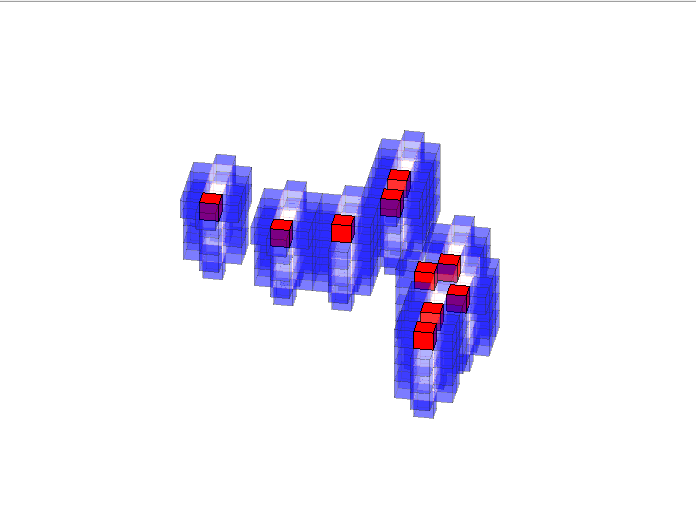
\includegraphics[height=0.2\paperheight]{3d1.png}
	\caption{The 3D simulation is shown above with red blocks being the particles, blue being the frontier cells, and white being free explored cells.}
	\includegraphics[height=0.2\paperheight]{10particles_720free.jpg}
	\caption{Here are 10 particles that have completed explored the same workspace shown in Fig. 1. As shown, the workspace is four rectangular boxes alternately added together.}
	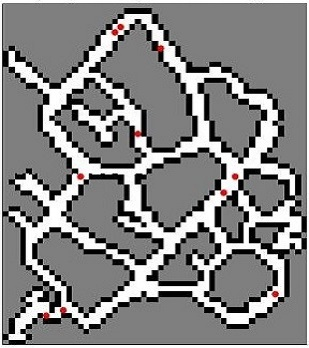
\includegraphics[height=0.2\paperheight]{10particles_final.jpg}
	\caption{For an equivalent 720 free cells in 2D, more moves were required by the ClosestFrontier Algorithm due to the increased complexity of this vascular system based off of a leaf tissue sample.}
\end{figure}
\bibliographystyle{IEEEtran}
\bibliography{abstract}

\end{document}
